\documentclass{ximera}

 

\usepackage{epsfig}

\graphicspath{
  {./}
  {figures/}
}

\usepackage{morewrites}
\makeatletter
\newcommand\subfile[1]{%
\renewcommand{\input}[1]{}%
\begingroup\skip@preamble\otherinput{#1}\endgroup\par\vspace{\topsep}
\let\input\otherinput}
\makeatother

\newcommand{\includeexercises}{\directlua{dofile("/home/jim/linearAlgebra/laode/exercises.lua")}}

%\newcounter{ccounter}
%\setcounter{ccounter}{1}
%\newcommand{\Chapter}[1]{\setcounter{chapter}{\arabic{ccounter}}\chapter{#1}\addtocounter{ccounter}{1}}

%\newcommand{\section}[1]{\section{#1}\setcounter{thm}{0}\setcounter{equation}{0}}

%\renewcommand{\theequation}{\arabic{chapter}.\arabic{section}.\arabic{equation}}
%\renewcommand{\thefigure}{\arabic{chapter}.\arabic{figure}}
%\renewcommand{\thetable}{\arabic{chapter}.\arabic{table}}

%\newcommand{\Sec}[2]{\section{#1}\markright{\arabic{ccounter}.\arabic{section}.#2}\setcounter{equation}{0}\setcounter{thm}{0}\setcounter{figure}{0}}

\newcommand{\Sec}[2]{\section{#1}}

\setcounter{secnumdepth}{2}
%\setcounter{secnumdepth}{1} 

%\newcounter{THM}
%\renewcommand{\theTHM}{\arabic{chapter}.\arabic{section}}

\newcommand{\trademark}{{R\!\!\!\!\!\bigcirc}}
%\newtheorem{exercise}{}

\newcommand{\dfield}{{\sf dfield9}}
\newcommand{\pplane}{{\sf pplane9}}

\newcommand{\EXER}{\section*{Exercises}}%\vspace*{0.2in}\hrule\small\setcounter{exercise}{0}}
\newcommand{\CEXER}{}%\vspace{0.08in}\begin{center}Computer Exercises\end{center}}
\newcommand{\TEXER}{} %\vspace{0.08in}\begin{center}Hand Exercises\end{center}}
\newcommand{\AEXER}{} %\vspace{0.08in}\begin{center}Hand Exercises\end{center}}

% BADBAD: \newcommand{\Bbb}{\bf}

\newcommand{\R}{\mbox{$\Bbb{R}$}}
\newcommand{\C}{\mbox{$\Bbb{C}$}}
\newcommand{\Z}{\mbox{$\Bbb{Z}$}}
\newcommand{\N}{\mbox{$\Bbb{N}$}}
\newcommand{\D}{\mbox{{\bf D}}}
\usepackage{amssymb}
%\newcommand{\qed}{\hfill\mbox{\raggedright$\square$} \vspace{1ex}}
%\newcommand{\proof}{\noindent {\bf Proof:} \hspace{0.1in}}

\newcommand{\setmin}{\;\mbox{--}\;}
\newcommand{\Matlab}{{M\small{AT\-LAB}} }
\newcommand{\Matlabp}{{M\small{AT\-LAB}}}
\newcommand{\computer}{\Matlab Instructions}
\newcommand{\half}{\mbox{$\frac{1}{2}$}}
\newcommand{\compose}{\raisebox{.15ex}{\mbox{{\scriptsize$\circ$}}}}
\newcommand{\AND}{\quad\mbox{and}\quad}
\newcommand{\vect}[2]{\left(\begin{array}{c} #1_1 \\ \vdots \\
 #1_{#2}\end{array}\right)}
\newcommand{\mattwo}[4]{\left(\begin{array}{rr} #1 & #2\\ #3
&#4\end{array}\right)}
\newcommand{\mattwoc}[4]{\left(\begin{array}{cc} #1 & #2\\ #3
&#4\end{array}\right)}
\newcommand{\vectwo}[2]{\left(\begin{array}{r} #1 \\ #2\end{array}\right)}
\newcommand{\vectwoc}[2]{\left(\begin{array}{c} #1 \\ #2\end{array}\right)}

\newcommand{\ignore}[1]{}


\newcommand{\inv}{^{-1}}
\newcommand{\CC}{{\cal C}}
\newcommand{\CCone}{\CC^1}
\newcommand{\Span}{{\rm span}}
\newcommand{\rank}{{\rm rank}}
\newcommand{\trace}{{\rm tr}}
\newcommand{\RE}{{\rm Re}}
\newcommand{\IM}{{\rm Im}}
\newcommand{\nulls}{{\rm null\;space}}

\newcommand{\dps}{\displaystyle}
\newcommand{\arraystart}{\renewcommand{\arraystretch}{1.8}}
\newcommand{\arrayfinish}{\renewcommand{\arraystretch}{1.2}}
\newcommand{\Start}[1]{\vspace{0.08in}\noindent {\bf Section~\ref{#1}}}
\newcommand{\exer}[1]{\noindent {\bf \ref{#1}}}
\newcommand{\ans}{}
\newcommand{\matthree}[9]{\left(\begin{array}{rrr} #1 & #2 & #3 \\ #4 & #5 & #6
\\ #7 & #8 & #9\end{array}\right)}
\newcommand{\cvectwo}[2]{\left(\begin{array}{c} #1 \\ #2\end{array}\right)}
\newcommand{\cmatthree}[9]{\left(\begin{array}{ccc} #1 & #2 & #3 \\ #4 & #5 &
#6 \\ #7 & #8 & #9\end{array}\right)}
\newcommand{\vecthree}[3]{\left(\begin{array}{r} #1 \\ #2 \\
#3\end{array}\right)}
\newcommand{\cvecthree}[3]{\left(\begin{array}{c} #1 \\ #2 \\
#3\end{array}\right)}
\newcommand{\cmattwo}[4]{\left(\begin{array}{cc} #1 & #2\\ #3
&#4\end{array}\right)}

\newcommand{\Matrix}[1]{\ensuremath{\left(\begin{array}{rrrrrrrrrrrrrrrrrr} #1 \end{array}\right)}}

\newcommand{\Matrixc}[1]{\ensuremath{\left(\begin{array}{cccccccccccc} #1 \end{array}\right)}}



\renewcommand{\labelenumi}{\theenumi)}
\newenvironment{enumeratea}%
{\begingroup
 \renewcommand{\theenumi}{\alph{enumi}}
 \renewcommand{\labelenumi}{(\theenumi)}
 \begin{enumerate}}
 {\end{enumerate}\endgroup}



\newcounter{help}
\renewcommand{\thehelp}{\thesection.\arabic{equation}}

%\newenvironment{equation*}%
%{\renewcommand\endequation{\eqno (\theequation)* $$}%
%   \begin{equation}}%
%   {\end{equation}\renewcommand\endequation{\eqno \@eqnnum
%$$\global\@ignoretrue}}

%\input{psfig.tex}

\author{Martin Golubitsky and Michael Dellnitz}

%\newenvironment{matlabEquation}%
%{\renewcommand\endequation{\eqno (\theequation*) $$}%
%   \begin{equation}}%
%   {\end{equation}\renewcommand\endequation{\eqno \@eqnnum
% $$\global\@ignoretrue}}

\newcommand{\soln}{\textbf{Solution:} }
\newcommand{\exercap}[1]{\centerline{Figure~\ref{#1}}}
\newcommand{\exercaptwo}[1]{\centerline{Figure~\ref{#1}a\hspace{2.1in}
Figure~\ref{#1}b}}
\newcommand{\exercapthree}[1]{\centerline{Figure~\ref{#1}a\hspace{1.2in}
Figure~\ref{#1}b\hspace{1.2in}Figure~\ref{#1}c}}
\newcommand{\para}{\hspace{0.4in}}

\renewenvironment{solution}{\suppress}{\endsuppress}

\ifxake
\newenvironment{matlabEquation}{\begin{equation}}{\end{equation}}
\else
\newenvironment{matlabEquation}%
{\let\oldtheequation\theequation\renewcommand{\theequation}{\oldtheequation*}\begin{equation}}%
  {\end{equation}\let\theequation\oldtheequation}
\fi

\makeatother


\title{The Continuous Flow Stirred Tank Reactor}

\begin{document}
\begin{abstract}
\end{abstract}
\maketitle

 
\label{S:CSTR} \index{CSTR}

Perhaps the simplest chemical engineering model of a chemical
reaction is the CSTR --- the continuous flow stirred tank
chemical reactor.  In the CSTR we imagine that a reactant flows
into a vessel and undergoes a single heat producing reaction to
form inert products.  The concentration of the reactant inside
the vessel is denoted by $c$ and the temperature of the fluid
inside the vessel is denoted by $T$.  The assumption that the
tank is well stirred is interpreted mathematically to mean that
$c$ and $T$ are constant everywhere in the vessel.  The CSTR
model describes how $c$ and $T$ evolve in time. 

The CSTR is pictured schematically in Figure~\ref{F:CSTRs}.  We assume 
that the reactant flows into a unit volume vessel at a constant rate 
$r$ and that the product flows out of the vessel at the same rate.  
The fluid that flows into the vessel is called the {\em feed\/}.  
We assume that the temperature of the feed is held constant at
$T_f$ and that the reactant concentration of the feed is $c_f$.
We also assume that the vessel is surrounded by a coolant whose
temperature $T_c$ is held constant.  

\begin{figure}[htb]
           \centerline{%
	   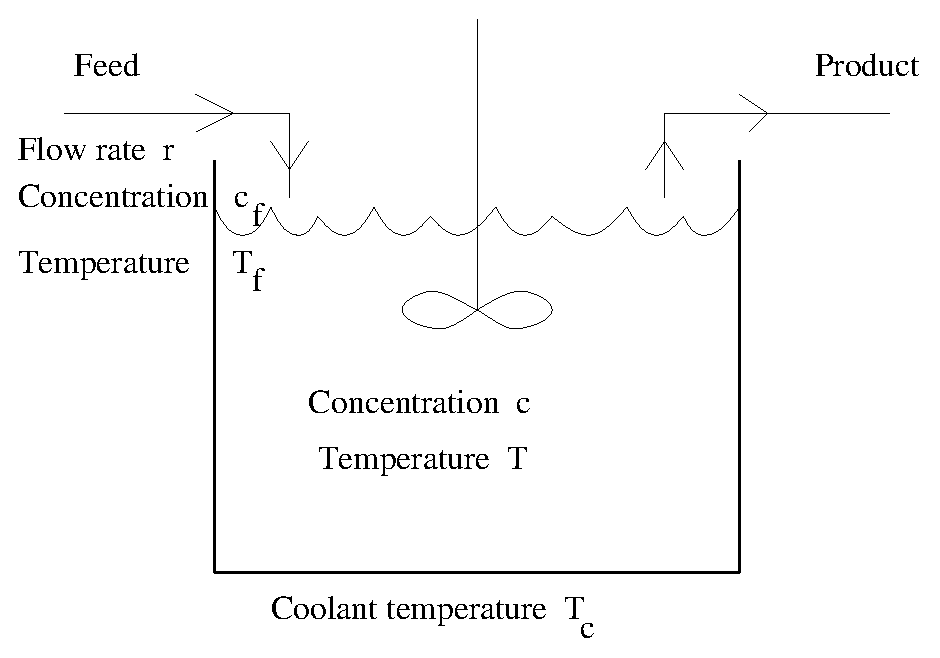
\psfig{file=../figures/CSTR.eps,height=3.0in}}
           \caption{Schematic diagram for CSTR.}
           \label{F:CSTRs}
\end{figure}\index{CSTR}


\subsection*{The Reactionless CSTR}
\index{CSTR}

Ignoring the effects of the chemical reaction, the model
equations describing the time evolution of the temperature and
concentration of the reactant in the vessel are:
\arraystart
\begin{equation} \label{e:CSTRlin}
\begin{array}{rcl}
\dps\frac{dc}{dt} & = & r(c_f-c) \\
\dps\frac{dT}{dt} & = & r(T_f-T) + k(T_c-T),
\end{array}
\end{equation}
\arrayfinish   \index{CSTR} 
where $k$ is a lumped parameter that depends on a variety of
physical quantities including heat transfer area and specific
heat.  

So far, the model in \eqref{e:CSTRlin} is an inhomogeneous uncoupled system
of linear differential equations.  We have assumed that the concentration 
of the reactant grows exponentially to the feed concentration at rate
$r$.  The fate of the temperature inside the vessel is less
clear, as we have assumed that the temperature grows exponentially to 
the feed temperature at rate $r$ and simultaneously grows
exponentially to the coolant temperature at rate $k$ (that is
just Newton's law of cooling\index{Newton's law of cooling}).  
At this point, we have not modeled the effects of the chemical reaction 
on concentration and temperature inside the vessel --- though we have modeled 
how the external variables such as feed temperature and concentration and 
the coolant temperature affect the concentration and temperature inside the 
vessel.  For this reason, this model is called the {\em reactionless\/} CSTR. 
Before continuing with the modeling, we 
nondimensionalize\index{nondimensionalize} the variables, as 
engineers prefer to do.

In this model, we have assumed implicitly that concentration and
temperature are positive quantities.  For concentration this is
clearly a reasonable assumption.  For temperature this means
that we are measuring temperature from absolute zero.  Suppose
that we let  \index{scaling}
\[
x(t) = \frac{c(\frac{t}{k})-c_f}{c_f} \AND 
y(t) = \frac{T(\frac{t}{k})-T_f}{T_f}
\]
be scaled concentration and temperature.  We have normalized $x$
and $y$ to measure deviation from the feed concentration and
temperature, and we have scaled $c$ and $T$ by $c_f$ and $T_f$
so that the state variables $x$ and $y$ are nondimensional ---
they have no physical units attached to them.  In addition, we
have scaled time by the lumped rate constant $k$.  (Chemical engineers
do not usually scale time in the equations, since $k$ is a 
parameter that can be controlled in experiments.) Next, let 
\[
\eta = \frac{T_c-T_f}{T_f} \AND \rho = \frac{r}{k}
\]
be the nondimensionalized coolant temperature and flow rate,
respectively.  Note that the fact that all physical quantities
were assumed to be positive leads to the restrictions
\[
x, y,\eta >-1  \AND \rho>0.
\]

Observe that 
\[
\frac{dx}{dt}(t)=\frac{1}{kc_f}\frac{dc}{dt}\left(\frac{t}{k}\right) \AND
\frac{dy}{dt}(t)=\frac{1}{kT_f}\frac{dT}{dt}\left(\frac{t}{k}\right).
\]
Coupling this observation with \eqref{e:CSTRlin} yields the equations 
for the reactionless CSTR in nondimensionalized form:
\begin{eqnarray}
\dot{x} & = & -\rho x \label{e:ndCSTRlina} \\
\dot{y} & = & -(\rho+1)y + \eta. \label{e:ndCSTRlinb}
\end{eqnarray}\index{CSTR}
The solution to \eqref{e:ndCSTRlina} is 
\[
x(t) = e^{-\rho t}x_0,
\]
and, in the absence of a reaction, the scaled concentration
decays exponentially to $x=0$, that is, to the feed
concentration.

The solution to \eqref{e:ndCSTRlinb} is slightly more complicated
to obtain in closed form, as this is an example of an
inhomogeneous linear equation.  Using 
superposition\index{superposition}, we can find
the general solution to the inhomogeneous equation by finding
one solution to the inhomogeneous\index{inhomogeneous} 
equation and adding in all
solutions to the homogeneous\index{homogeneous} equation.  
In this case, it is easy to find a constant solution to the 
inhomogeneous equation.  Just set
\begin{equation}  \label{e:basetemp}
y = \frac{\eta}{\rho+1},
\end{equation}
and check that this constant is a solution to
\eqref{e:ndCSTRlinb}.  As we know,
\[
y(t) = e^{-(\rho+1)t}K
\]
is the general solution to the homogeneous equation, and
\[
y(t) = e^{-(\rho+1)t}K + \frac{\eta}{\rho+1}
\]
is the general solution to \eqref{e:ndCSTRlinb}.  Thus,
temperature decays exponentially to \eqref{e:basetemp}, the
coolant temperature in nondimensionalized form scaled by the
nondimensionalized flow rate\index{flow rate}.

\subsection*{The CSTR}
\index{CSTR}
 
Next we consider the effects of the reaction.  For thermodynamic
reasons, which we do not discuss here, we assume that the
reaction depletes the reactant at a temperature dependent rate
proportional to concentration times the {\em Arrhenius\/} term
\index{Arrhenius term} $A(y)$ where
\[
A(y) = \exp\left(\frac{\gamma y}{y+1}\right)
\]
and $\gamma$ is the {\em activation 
energy\/}\index{activation energy}.  Since the
reaction is heat producing, we also assume that the temperature
of the reactant increases at a rate proportional to $cA(y)$.
Since the concentration $c$ is proportional to $x+1$, these
assumptions lead to the nonlinear system of differential
equations
\begin{matlabEquation} \label{e:CSTR}
\begin{array}{rcl}
\dot{x} & = & -\rho x  - Z(x+1)A(y) \\
\dot{y} & = & -(\rho+1)y + \eta + hZ(x+1)A(y),
\end{array}
\end{matlabEquation}
where $Z$ and $h$ are proportionality constants.  In this form
the equations have two state variables $x,y$ and five constants
$\rho,\eta,\gamma,Z,h$.  (The CSTR equation in {\tt e12\_3\_5.pps} has
$\gamma=4$ so that there are just four parameters.)

\subsection*{Numerical Solution of the CSTR}
\index{CSTR}

It is a difficult problem to determine the phase portraits for
the CSTR equations for all values of the five constants. Here we
use {\sf pplane8} to indicate some of the different phase
portraits that can occur in these equations.  In order to
simplify the task, we fix values for all parameters except
the nondimensionalized flow rate $\rho$.  We set
\begin{equation}   \label{e:CSTRparam}
\gamma=4, \quad \eta=-0.75, \quad Z=0.5, \quad h =3.
\end{equation}
Numerical experimentation on the rectangle $-0.75\leq x
\leq 0.5$, $-0.75\leq y\leq 0.75$ shows the following.  There are 
three possible equilibria --- one at high temperature ($y\sim 0.1$), 
one at medium temperature ($y\sim -0.1$), and one at low
temperature ($y\sim -0.5$).  For these parameter values, the 
equilibrium at medium temperature is always a saddle and the 
equilibrium at low temperature is always a 
sink\index{sink}.  We present the 
phase portraits for five values of the nondimensionalized 
flow rate\index{flow rate}
$\rho$.  The results are as follows:  
\begin{itemize}
\item[$\rho=0.495$] The only equilibrium is the low temperature 
equilibrium and it is a nodal sink. 
\item[$\rho=0.520$] There are three equilibria. The high 
temperature spiral source and the medium temperature saddle appear
as $\rho$ is increased.  Note that the stable orbit of the 
saddle connects directly to the spiral source.
\item[$\rho=0.545$] The high temperature equilibrium is a spiral 
sink and the stable orbit of the saddle connects to a limit 
cycle.  At this parameter value, there are two stable equilibria.
\index{limit cycle} \index{stable!orbit}
\item[$\rho=0.570$] There are still three equilibria, but the 
time-periodic solution has disappeared.  The unstable orbit of 
the saddle now connects to the high temperature spiral sink. The
low temperature sink is a spiral sink and there are two stable
spiral sinks. 
\item[$\rho=0.720$] The only remaining equilibrium is the high
temperature spiral sink.  The saddle and the low temperature 
sink have coalesced and disappeared.  (Presumably the low temperature 
spiral sink became a nodal sink before it coalesced with the saddle.)
\end{itemize}

These calculations show that the phase portrait of the CSTR changes 
between successive values of $\rho$, that is, we have shown that 
there are at least four bifurcation values in the CSTR as $\rho$ 
is varied.  The five different phase planes are shown in Figure~\ref{F:CSTR}.


\begin{figure}
           \centerline{%
	   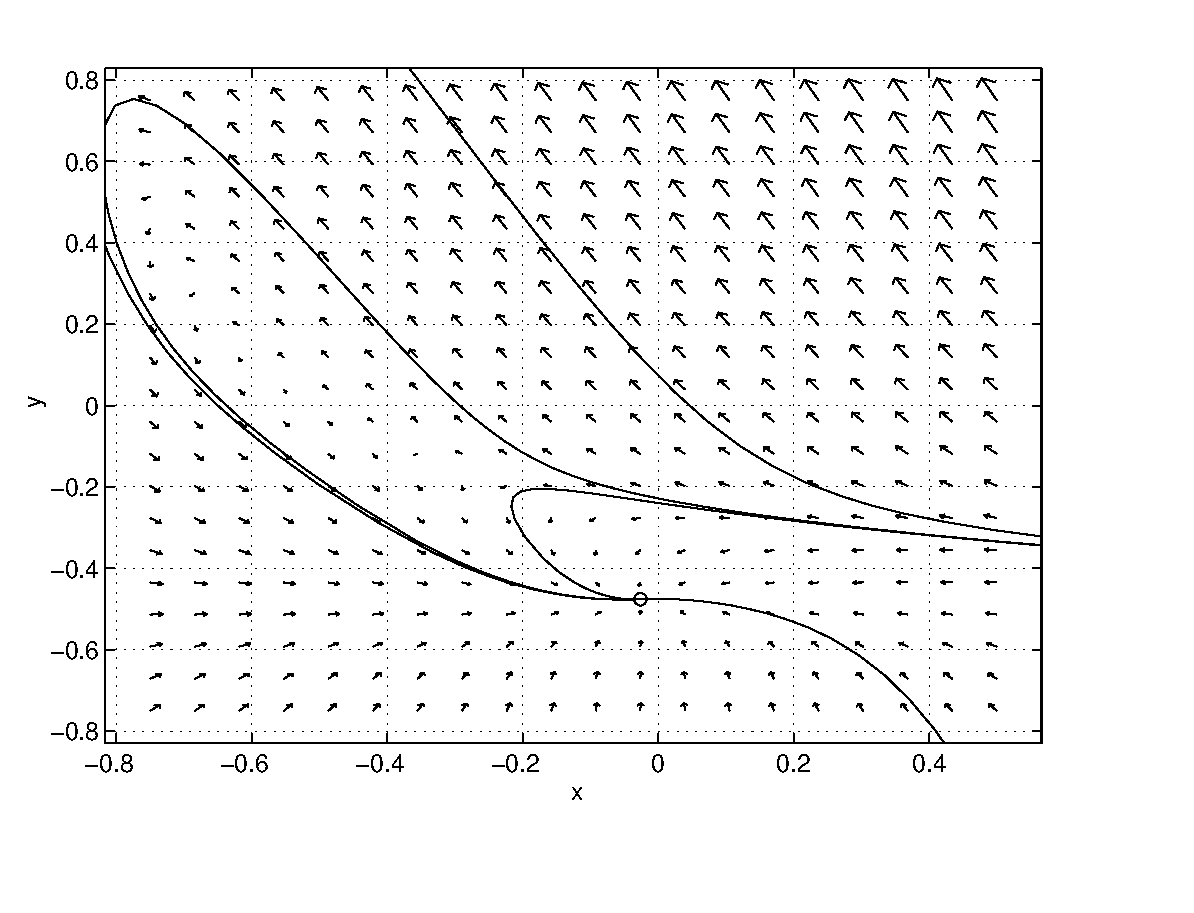
\psfig{file=../figures/cstr495.eps,height=2.1in}
	   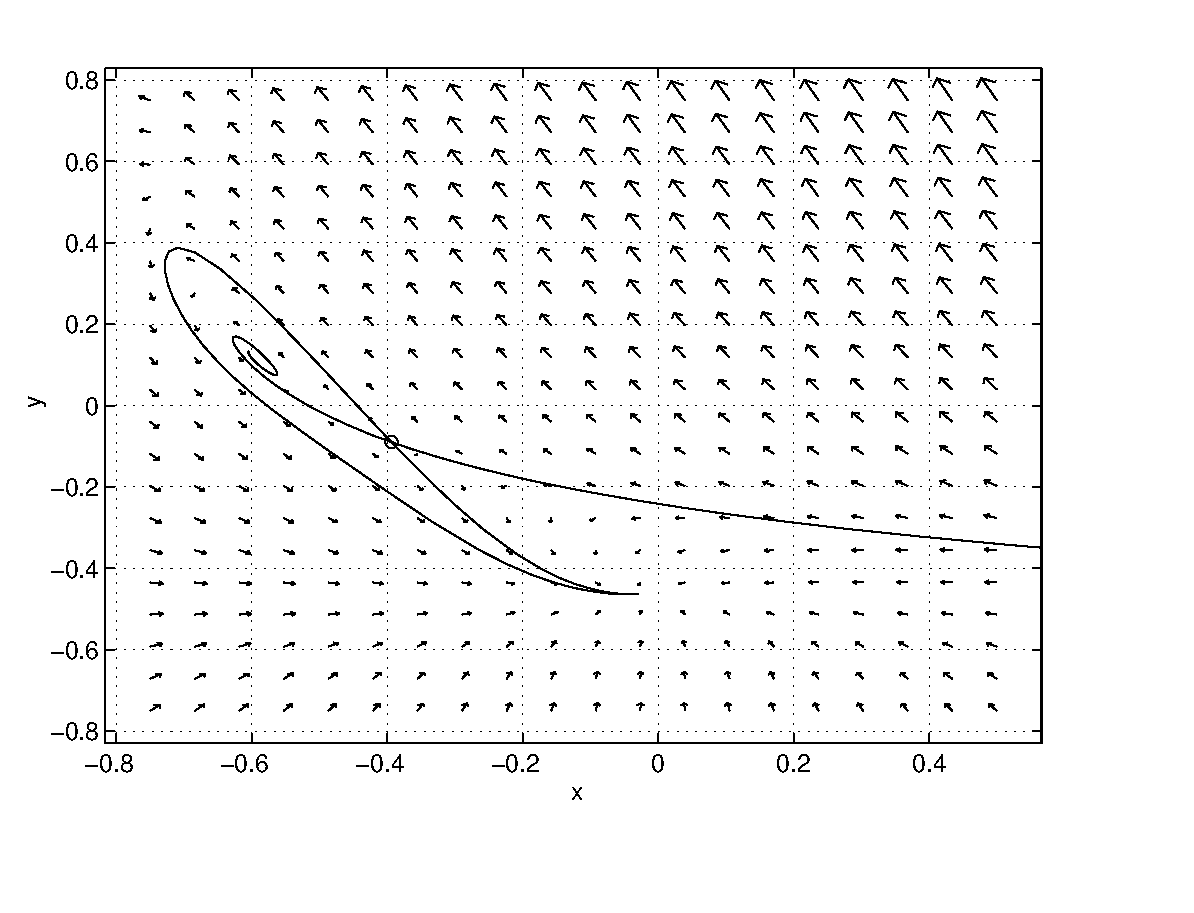
\psfig{file=../figures/cstr52.eps,height=2.1in}}	
		\vspace*{-0.2in}	
		$\hspace{1.2in} \mbox{$\rho=0.495$ \hspace{2.0in} $\rho=0.52$}$
           \centerline{%
	   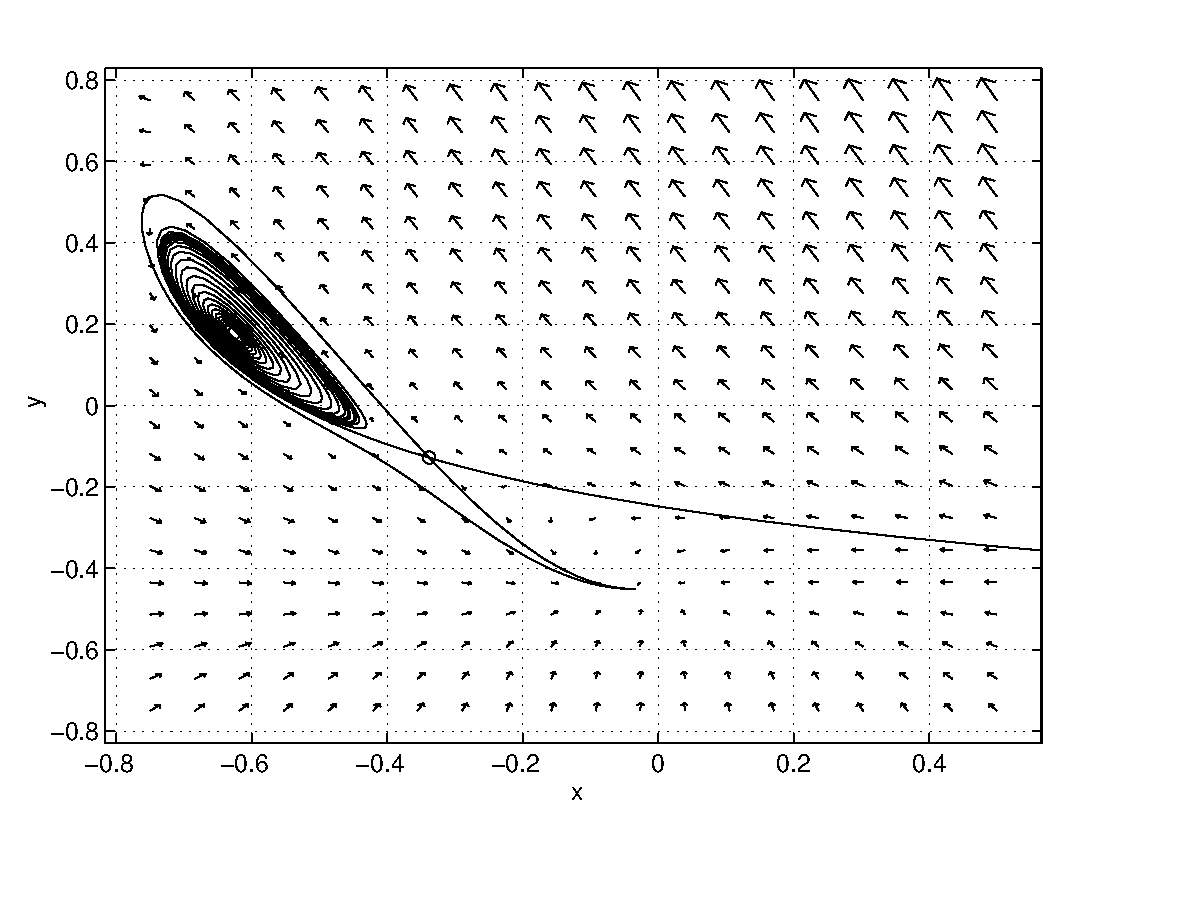
\psfig{file=../figures/cstr545.eps,height=2.1in}
	   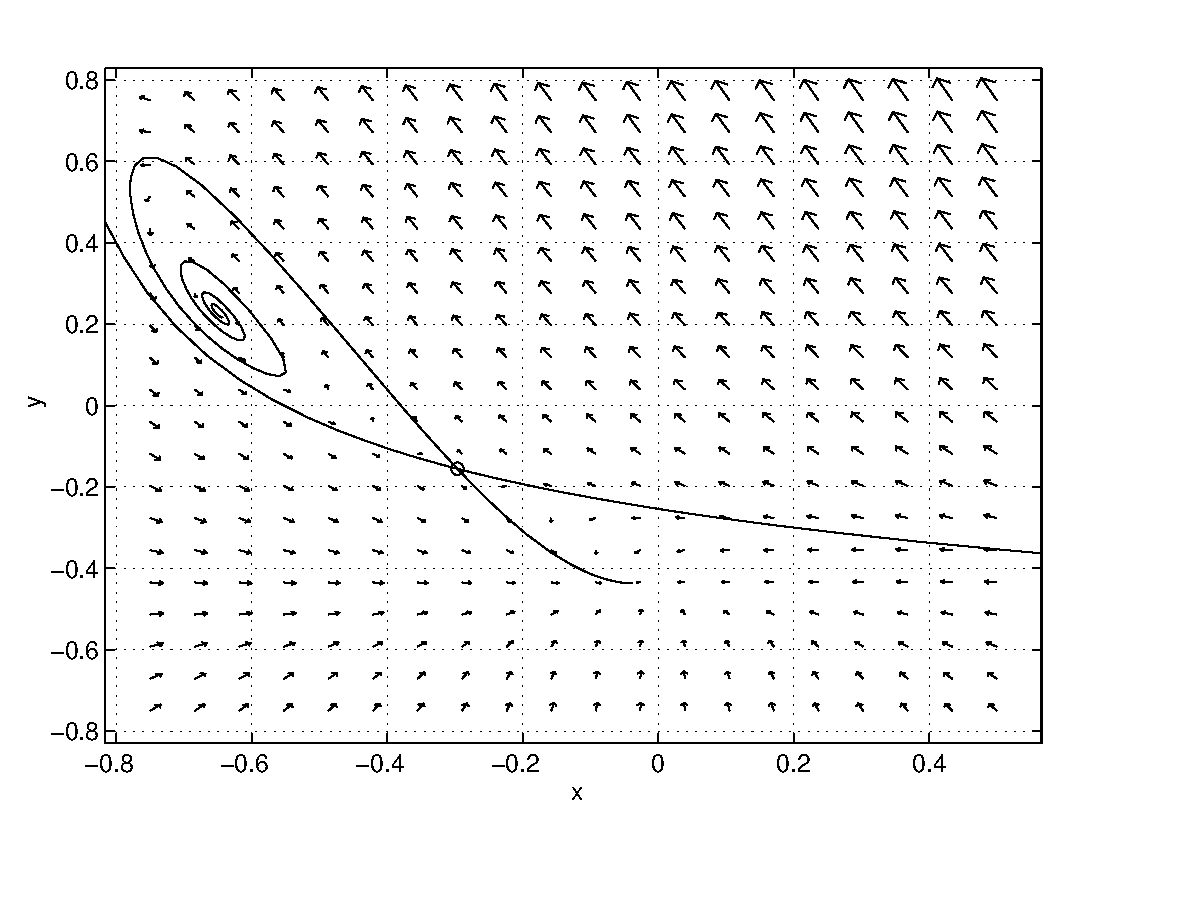
\psfig{file=../figures/cstr57.eps,height=2.1in}}
		\vspace*{-0.4in}
		
		$\hspace{1.2in} \mbox{$\rho=0.545$ \hspace{2.0in} $\rho=0.57$}$
		\vspace{0.4in}
	   \centerline{%
           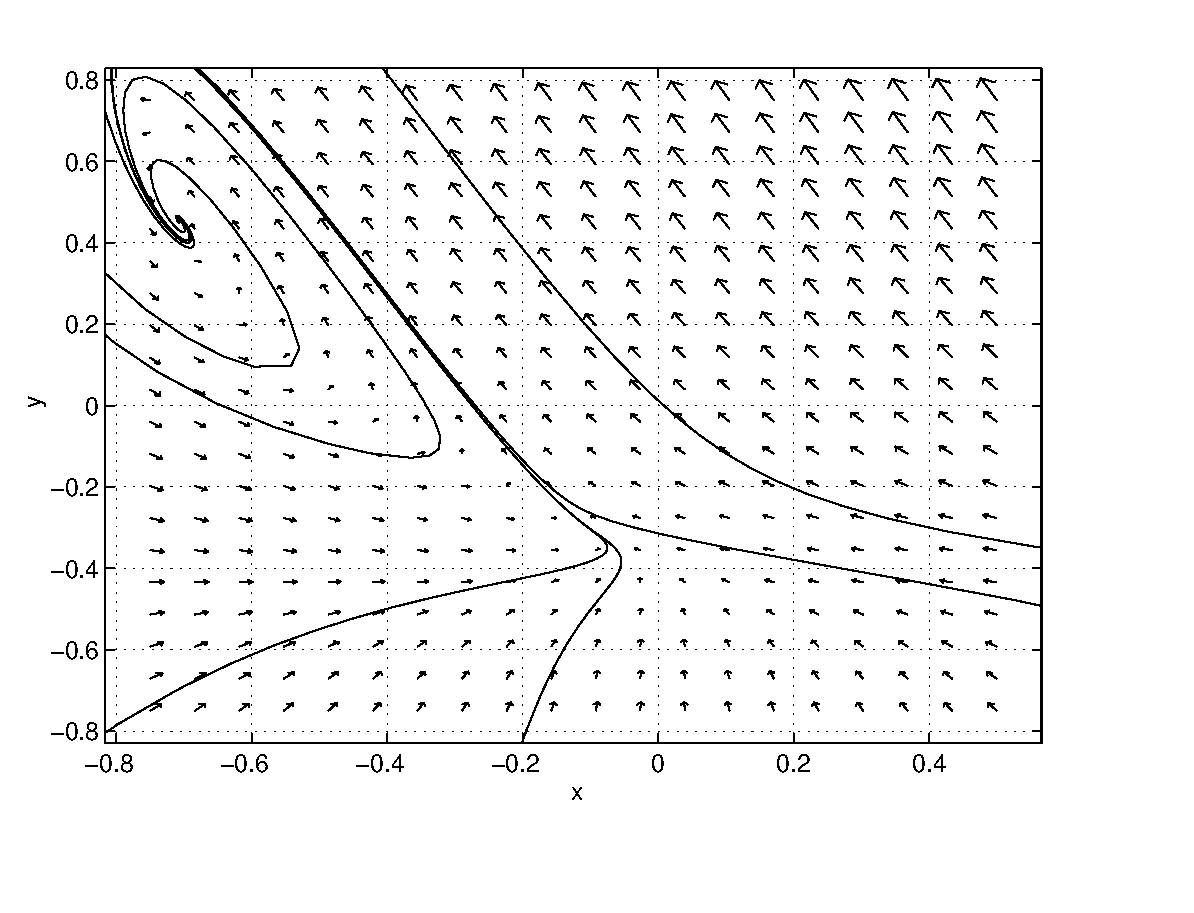
\psfig{file=../figures/cstr72.eps,height=2.1in}}
 		\vspace*{-0.8in}
		
		\hspace{2.6in} $\rho=0.72$
          \caption{Phase portraits of CSTR \protect\eqref{e:CSTR} 
	with $\gamma=4$, $\eta=-0.75$, $Z=0.5$, $h =3$.}
           \label{F:CSTR}
\end{figure}


\subsection*{Bifurcations in the CSTR}
\index{CSTR}


The observed bifurcations in the CSTR divide into local and global 
bifurcations, as we now discuss.

As we saw in Section~\ref{S:bifurcation}, local bifurcations are of two 
types: steady-state (saddle-node) and Hopf. \index{bifurcation!steady-state} 
\index{bifurcation!Hopf}  For example, in Figure~\ref{F:CSTR}, we see that as 
the parameter $\rho$ is decreased from $0.52$ to $0.495$ the middle and high 
temperature equilibria collide and disappear at a saddle-node bifurcation.  
See Exercise~\ref{E:CSTR5} for further verification of this fact.  Similarly,
between the values of $\rho=0.57$ and $\rho=0.72$ the low and middle 
temperature equilibria collide and disappear.  We presume that a  
saddle-node bifurcation has also occurred in this parameter regime.

A different bifurcation occurs as $\rho$ increases from
$0.52$ and $0.545$.  In this range, the high temperature spiral
changes from a source to a sink.  For this change to occur,
there must be a parameter value where the high temperature
equilibrium is a center.  Since a time periodic solution
is found in the phase portrait of the CSTR at $\rho=0.545$, we 
conclude that a Hopf bifurcation has occurred in this parameter region.

Both of these local bifurcations occur at parameter values where
there is a nonhyperbolic equilibrium. As we noted, Hopf
bifurcation occurs at a parameter value where a center is
present, while steady-state bifurcation occurs at a parameter value where 
an equilibrium has a Jacobian matrix with a zero eigenvalue --- typically 
a saddle-node.  

A global bifurcation\index{bifurcation!global}, one in which the bifurcation
in phase portraits occurs away from equilibria, is present in the CSTR 
between $\rho=0.545$ and $\rho=0.57$.  In this region, the periodic solution 
grows until it touches the saddle point.  At that point, one branch of 
the stable orbit and one branch of the unstable orbit of the 
saddle are identical.  Thus, there is a trajectory that limits
on the saddle point in both forward and backward time.  As we 
saw in Section~\ref{S:bifurcation} such trajectories are called 
{\em homoclinic\/} trajectories and such bifurcations are called 
{\em homoclinic bifurcations\/}.  \index{trajectory!homoclinic} 
\index{bifurcation!homoclinic}  Note the similarity between the phase 
portraits in Figure~\ref{F:homobif} and the middle phase portraits in 
Figure~\ref{F:CSTR}.

There are other global bifurcations that we have not seen in 
these equations.  Two periodic solutions can collide and both 
disappear (just like the saddle-node steady-state bifurcation 
where two equilibria collide and disappear).  This bifurcation is
discussed in Section~\ref{S:GlobalBif}.  Another global 
bifurcation occurs when the stable orbit of one saddle point 
coincides with the unstable orbit of another saddle point.  
This bifurcation is called a {\em saddle-saddle\/} connection.  
The homoclinic bifurcation is a special case of a saddle-saddle 
connection where the two saddle points are the same.
\index{saddle-saddle connection}  See Section~\ref{S:bifurcation}.

\subsection*{Bifurcation Diagrams}
\index{diagram!bifurcation}

The discussion of transitions in the 
CSTR\index{CSTR} can be summarized by the use of a 
{\em bifurcation diagram\/}, as introduced in Section~\ref{S:bifurcation}.  
In a bifurcation diagram we graph the equilibria {\em and\/} periodic 
solutions of equations as a function of the parameter $\rho$.  In 
bifurcation diagrams: \index{diagram!bifurcation}
\begin{itemize}
\item	A saddle-node bifurcation appears as a turning point in 
	a branch of equilibria.
\item	A Hopf bifurcation appears as a change in stability along 
	a branch of equilibria.
\item	A homoclinic bifurcation is noted by a sudden ending of a 
	branch of periodic solutions.
\end{itemize}
In the CSTR equations we have numerical evidence for two saddle-node 
bifurcations, a Hopf bifurcation, and a homoclinic bifurcation.  
This information is illustrated in the bifurcation diagram in 
Figure~\ref{F:CSTRbif}.  Bifurcation diagrams contain an enormous amount 
of information --- and it takes practice to learn to read them.  For 
example, suppose $\rho$ is fixed to be $0.545$ in Figure~\ref{F:CSTRbif}.
Then we may surmise that there are three equilibria of the CSTR equations
at that value of $\rho$ --- the low and high temperature equilibria are 
asymptotically stable while the middle temperature one is not --- and an 
unstable limit cycle (that surrounds the high temperature equilibrium).

\begin{figure}[htb]
           \centerline{%
	   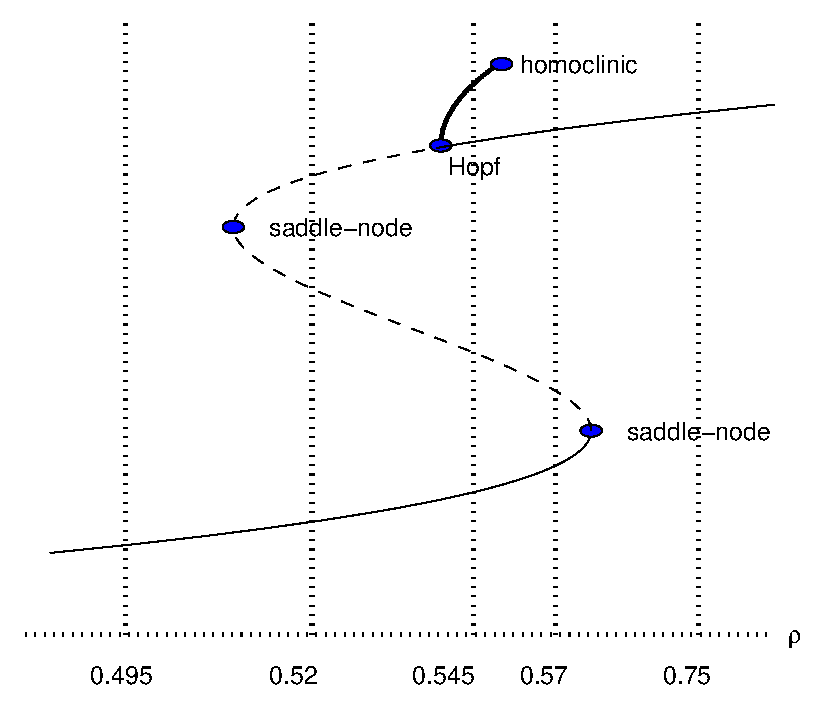
\psfig{file=../figures/cstrbif.eps,width=4.0in}}
           \caption{Schematic bifurcation diagram for the CSTR}
           \label{F:CSTRbif}
\end{figure}


\EXER

\CEXER

\begin{exercise}  \label{E:CSTR5}
Consider the CSTR equations \eqref{e:CSTR} with parameters 
\eqref{e:CSTRparam}. Set $\rho=0.5$ and use 
{\sf pplane8}\index{\computer!pplane8} to verify 
that there are two equilibria --- a low temperature nodal sink 
and a middle temperature saddle-node equilibrium.  Then change 
$\rho$ to $0.505$ and verify that the saddle-node has split 
into two equilibria --- a saddle and a spiral source.
\end{exercise}

\begin{exercise} \label{c9.2.2}
Use {\sf pplane8} to explore the CSTR equations \eqref{e:CSTR} with
parameters:
\[
h=2, \quad Z=0.5, \quad \eta=-0.5, \quad \gamma=5,
\]
for various values of the parameter $\rho$ between $0.46$ and 
$0.51$.  Describe all equilibria and all periodic solutions that 
you find, and how they change as $\rho$ is varied.
\end{exercise}



\end{document}
